\section{Introduction}
\label{sec:introduction}
% This introduction outlines the sections of our document, outlines what we hope to accomplish and outlines how we will do it (i.e. our methods).
% The first paragraph is an overview of our topic
Our project aims to examine whether online petitions can be effective in driving social change for environmental protection. Macionis and Plummer address digital democracies by suggesting that new social movements based on online communication are partly reshaping politics \citep[Chap. 23]{Plummer11}. Our project will show the extent to which this is occurring, focusing especially on how online petitions from seemingly `powerless' individuals have amassed hundreds of thousands of supporters across the globe and appear to result in political and corporate action in areas of environmental protection and many others. Our project aims to test this theory using Change.org as our primary case study, academic literature and other sources.\par\vspace{0.2cm}

Change.org is a for-profit, socially-oriented business running a website where, at no cost, anyone can start an online-petition to raise support on for a given issue. Change.org states its mission as ``empowering people everywhere to create the change they want to see'' \citep{Change14a}.  It is tackling the problem of how communities can speak to their politicians and economic leaders. It gives a voice to those who are experiencing the consequences of government action or economic inequalities to speak up and garner support from a large community to address the issue. The service is used by ``more than 65 million users in 196 countries ... to transform their communities -- \textbf{locally, nationally and globally}'' \citep{Change14a}.  We will be looking particularly at how effective this online tool is at \textbf{creating social movements around environmental protection initiatives}.\par\vspace{0.2cm}

The main hypothesis tested by the research presented in this paper is as follows:

\begin{hyp}
\item Online petitions drive social change in favour of protecting the environment.
\end{hyp}

% This second introductory paragraph outlines the sections of our document
\subsection{Outline}
\label{subsec:outline}
Firstly, this paper puts the project into the context of the current interplay between the \textbf{tools of digital democracies} and \textbf{environmental protection} in The Big Idea section. Additionally, we introduce key theories about the current state of the environment, digital democracies and social movements. Following The Big Idea section is the Methods section, describing the literature reviews, online petition case studies, interviews and surveys used to substantiate our analysis, both conducted and proposed. Finally, the Conclusion section arrives at a judgement of whether online petitions do indeed drive social change in favour of protecting the environment.

\subsection{Objectives}
\label{subsec:objectives}
The \textbf{strategic objective} we want to achieve with our work is to inspire more people to engage with digital democracy. To reach this target we will build up a belief in digital democracy (\textbf{tactical level}) by evaluating famous examples and analysing the existing tools allowing participation in digital democracy (\textbf{operational level}). As a result of this analysis we want people to engage with digital democracy (\textbf{tactical level}) by showing them what make critical success factors for such initiatives (\textbf{operational level}). Lastly, in terms of environmental protection, there is a need to drive the initiatives from a local to a global level (\textbf{tactical level}).\par\vspace{0.2cm}
The following mind maps visualise the hierarchy of objectives. The black node represents strategic levels, the blue nodes tactical levels and the green nodes operative levels. \\
\begin{figure}[H]
\resizebox{1.1\textwidth}{!}{
\begin{tikzpicture}
  \path[mindmap,grow cyclic,every node/.style=concept, concept color=black!75!white,text=white, 
    level 1/.append style={concept color=green!40!blue,level distance=140,sibling angle=120,},
    level 2/.append style={concept color=green!50!blue,level distance=110,sibling angle=60},]
   
    node[] {Inspire more people to engage with digital democracy}
    [clockwise from=45]
		child[] {node[] {build up belief in digital democracy}
        [clockwise from=90] 
        	child[] {node[] {evaluate famous examples}}
            child[] {node[] {analyse online petition systems}}
        }
        child[] {node[] {engage people into digital democracy}
        	[clockwise from=-50]
        	child[] {node[] {analyse success factors}}
            child[] {node[] {how and when to use each system}}
            %child[] {node[] {...}}
        }             
        child[] {node[] {drive initiatives from local to global level}        	
        	[clockwise from=-120]
            child[] {node[] {reach a wider audience}}
            child[] {node[] {connect to real world}}
        }
    ;
\end{tikzpicture}
}
\caption{Mind map: Inspire more people to engage with digital democracy}
\end{figure}
\subsection{Priorities of Objectives}
Ultimately, we would like to shine the spotlight on digital democracy by examining how effective online petitions are at driving political action. Therefore, our highest priority is to demonstrate the effectiveness of such tools as stated in the operative objective: `evaluating famous examples'. Secondly, taking another operative objective, we would like to identify tools that are readily accessible to readers, thereby encourage engagement with digital democracy. Following these priorities, we aim to examine how local initiatives can drive global action. In order, our priorities are:

\begin{enumerate}
	\item Highest Priorities
    \begin{enumerate}
        \item \emph{Operative objective}: Evaluate famous examples
    	\item \emph{Tactical objective}: Build up belief in digital democracy
  	\end{enumerate}
	\item High Priority
	\begin{enumerate}
	    \item \emph{Operative objective}: Demonstrate tools such as Change.org
	    \item \emph{Operative objective} Outline how the tools can be utilised
    	\item \emph{Tactical objective}: Encourage engagement with digital democracy
  	\end{enumerate}
  	\item Moderate Priority
  	\begin{enumerate}
  	    \item \emph{Operative objective}: Demonstrate how online petitions connect to real-world action and environmental issues.
  	    \item \emph{Operative objective}: Show how online petitions reach a global audience.
  	\end{enumerate}
    \item Low Priority
    \begin{enumerate}
        \item \emph{Strategic objective}: Inspire more people to engage with digital democracy
    \end{enumerate}
\end{enumerate}

Although, the lowest priority is the sole strategic objective, it should be also noted that the priority list puts operative objectives first. We have placed the highest importance on laying down a solid foundation for which our higher-level objectives can be built upon. Furthermore, endeavouring to inspire people to engage with digital democracy would indicate we find a positive result prior to testing the effectiveness of online petitions. Instead, our higher priorities are operational tasks such as evaluating famous examples in order to keep an open mind to the possibility that online petitions are not effective in driving social change for the environment.
% subsection Our Objectives (end) 

\subsection{Scope}
\label{sec:scope}
As shown in our objectives, our primary focus is on addressing the effectiveness of online petitions in driving social change for environmental protection. We have limited our scope in the following ways in order to in order to target our analysis:

\begin{itemize}
  \item We will only analysing the effectiveness of online petitions. Other tools of digital democracies such as social networks, blogs, forums, micro-blogging sites, individual websites, open data and open knowledge portals, e-governments, e-voting and so on are outside the scope of this project.
  \item Use Change.org as the primary case study. Other online petition sites are generally outside the scope of our project, but may be considered as alternative models.
  \item Focus on issues of environmental protection. Online petitions for other issues such as public health, human rights, consumer rights and so on are also generally outside the scope of the project. However, some exceptional cases may be considered in order to compare characteristics of those online petitions to those of environmental petitions.
\end{itemize}

Essentially, this project examines the following questions:

\begin{enumerate}
    \item Are online petitions successful effective in protecting the environment?
    \item Are online petitions effective on local, national and global levels?
    \item What characteristics constitute a successful petition?
    \item How do online petitions generate real world change?
    \item How do online petitions differ from traditional petitions?
    \item What are the motivations of a corporation, like Change.org, in running an online petition service?
%    \item What defines a Benefit Corporation (B Corporation) and how does the business model work?
\end{enumerate}

% End of Scope Subsection
% End of Introduction Section

\section{The Big Idea}
\label{sec:bigIdea}
% introduce the context - what is happening in the environment, what is happening in social movements, what is happening with digital democracy, focusing on online petitions
There are three primary concepts in which the study of online petitions: digital democracy, environmental protection as a sociological problem and social change and social movements. This section looks at each of these in detail in order put the project into context.
\subsection{Forms of Digital Democracy}
\label{subsec:digdemocracy}
Presently, many new forms of collaboration and channels of communication are being invented and innovated upon. The Internet has changed the way information flows and how information is controlled (or not controlled). It has brought forth new tools of governance and making collective decisions. These tools can be unified under the term \textbf{digital democracy}. The Internet is utilized by politicians, journalists, entrepreneurs and other officials as well as citizens to support and capitalize on their ideas. In recognition of this facet of the Internet, it has been stated that ``the Internet is the most democratizing innovation we've ever seen, more so even than the printing press'' \citep[pg. 2]{Hindman09}. Traditional print media is especially challenged by the new medium as the Internet ``will give new voice to people who've felt voiceless'' \citep[pg. 2]{Hindman09}. Being able to participate in political discourses, stating opinions and publishing information on the Internet gives an increasingly large number of people ``a degree of empowerment they never had before'' \citep[pg. 2]{Hindman09}. This new medium has an impact on nearly every aspect of our daily life -- economically, socially, politically and in many other ways. When focusing on the political aspect it is assumed that \begin{quote}the Internet is redistributing political influence; it is broadening the public sphere, increasing political participation, involving citizens in political activities that were previously closed to them, and challenging the monopoly of traditional elites \citep[pg. 6]{Hindman09}\end{quote}Those assumptions hint at an underlying movement from a more traditional \textbf{power elite model} to a new \textbf{pluralist model}. Whereas in the former model the power is concentrated among the rich, who have an huge impact on the political decision making, the latter one puts the power into the hand of many competing interest groups and sees the political process as an ongoing negotiation between those groups \citep[pg. 550]{Plummer11}. Whether this new approach for political participation is already a reality and whether it impacts environmental protection case still has to be seen. Hence, the decision to undertake this project.\par\vspace{0.2cm}

Though all of the aforementioned benefits of the Internet as a new medium are commonly agreed upon it also enables new types of powerful individuals, organizations and social behaviours. Even if the \textit{production} of information has been more democratized by it there are still gatekeepers involved in \textit{filtering} and \textit{finding} the information available. Those gatekeepers usually personalize in form of the \textbf{search engines} and \textbf{social networks}. Search engines, for example, take the importance of a web site into account by analysing the number of hyperlinks pointing to it (among other factors). As the search engines usually decide what regular people find and see on the Internet the result is that\begin{quote}not all choices are equal. Some sites consistently rise to the top of Yahoo!'s and Google's search results; some sites never get indexed by search engines at all. The visibility of political content on the Internet follows winners-take-all patterns, with profound implications for political voice. \citep[pg. 15]{Hindman09}\end{quote}That also means there is a difference between those who are speaking and those who are being heard on the Internet. Just being able to share your view online is not sufficient. You also need to reach a large audience to get recognized on the Internet -- but here you will face ``plenty of formal and informal barriers ... most online content receives no links, attracts no eyeballs, and has minimal political relevance.'' \citep[pg. 18]{Hindman09}.\par\vspace{0.2cm}

Though the Internet has removed some existing political inequalities it also creates new ones due to its structure and operation. Those are largely problems of economics, in form of supporting commercial interests of companies like Google, Microsoft and Yahoo!, and social facets -- as most opinions on the Internet are created by a small group of white, highly educated, male professionals \citep[pg. 18f]{Hindman09}. \par \vspace{0.2cm}

By definition a digital democracy uses modern, digital technologies to assist members of the 'political or social unit' in the political process. Therefore the tools of digital democracies may have an important role to play to drive political action for environmental protection. With the advent of the Internet, local environmental issues can attract global attention through the use of those online tools. In the case of this project, we examine how an online petition allows anyone with Internet access to start a petition and attract electronic signatures from other users in support of a particular issue.\par \vspace{0.2cm}
% forms of digital democracy (end)

\subsection{Environmental Protection a sociological problem}
\label{subsec:environmentProblems}
Seemingly completely disconnected from the Internet's underpinning of digital democracy is the concept of the \textbf{natural environment} in the sociological context. The natural environment describes ``the earth's surface and atmosphere, including all living organism as well as the air, water, soil and other resources necessary to sustain life'' \citep[pg. 869]{Plummer11}. The natural environment is changing as a result of human activities, putting the topic into the focus of sociologists in the late 20$^{th}$ century. It is ``now apparent that any understanding of the natural environment and its problems must also be global in scope'' \citep[pg. 870]{Plummer11}.\par\vspace{0.2cm}

Today, Earth faces an increasing number of global environmental problems: excessive waste, climate change, the trend toward urbanisation and ever larger industrial production sites around the globe. As well as consuming the limited resources of the planet, these occurrences also pollute the air and water leading to higher temperatures and polar ice melting on earth \citep[pg. 876ff]{Plummer11}.\par\vspace{0.2cm}

The current environmental movement has its roots in the late 1960s \citep[p. 888]{Plummer11}. At that time, it aimed to change the attitudes of the people to adapt their daily routines into more sustainable directions by showing the impact of their actions on the environment. \citet{Plummer11} define several more iterations of the environmental movement in the subsequent decades. In its second iteration, the environmental movement took a more policy-oriented perspective with focus on legal and economic pay-off. This phase was primarily driven by experts and authorities with the focus of developing a solid basis for environmental policies and reforms. In the 1970s it was clear that information gaps, transaction costs and private ownership of information were the main reasons to blocking effective and efficient environmental policy making, implementation and control. During the 1980s a more critical view emerged based on the theory of the Risk Society \citep[pg. 7f]{Mol08}.\par\vspace{0.2cm}

The \textbf{Risk Society} theory is based on the idea that new technologies, that we introduce to fulfil a specific need or help to solve our current problems, will itself generate new kinds of issues of an even higher magnitude than ever before, not only for us but also for the whole planet. In contrast to previous risks that are mainly based on natural origins like earthquakes or floods, the new kind of ``manufactured risks'' are hard to predict and could have huge consequences in the long run for all living creatures on earth \citep[pg. 53]{Plummer11}.\par\vspace{0.2cm}

Conversely, discussions on environmental protection for many decision-makers and politicians are centred around a \textbf{technocentric view} on the topic by stating that new technologies that are currently developed or are still to be invented will help humankind to solve environmental problems in the future. This deceptively conservative point of view tries to maintain status quo, especially existing policies, and puts all hope to solve the environmental problems into the hands of future generations. \citep[pg. 891]{Plummer11}\par\vspace{0.2cm}

At the opposite end of the spectrum are the supporters of the \textbf{ecocentric view}. The ecocentric view asserts that there is a \textbf{limit to growth}, and adopting `technical and scientific solutions to the problems may just increase them', especially in regard to environmental objectives \citep[p. 891]{Plummer11}. The ecocentric view observes that there are many disadvantages when still relying on the logic of growth -- namely the limited resources of the earth, the amount of waste that is produced each year, the destruction of life-giving environments like the Amazon Rainforest as well as the complexity of today's technology that conceals the risks of its usage \citep[pg. 874]{Plummer11}. Supporters of the ecocentric view encourage a radical shift in economical and political behaviour to protect the environment and they do not trust nor rely on technological advances to solve environmental issues. \citep[pg. 891]{Plummer11}\par\vspace{0.2cm}

Additionally, the environmental problems also raise \textbf{ethical issues}. The current environmental problems are primarily caused by developed countries which both produce large amounts of waste and have large second-level industries expelling gas emissions into the atmosphere and disposing of pollutants into the rivers and oceans. As it has been established, the environmental is interconnected across the globe, so the waste generated also affects people living in the developing world -- and those are even more seriously impacted upon than the waste creators \citep[pg. 870ff]{Plummer11}.\par\vspace{0.2cm}

There is also a \textbf{political aspect} to consider as there is a growing realisation that global coordination, worldwide media campaigns and large monetary resources are required to solve the environmental problems. Furthermore, large scale environmental protection efforts need support from multiple governments, politic leaders and organisations. In the current international systems those efforts become part of political trades. These circumstances make it difficult to scale the initiatives required to solve the environmental problems on the planetary level. A well-known example of such intergovernmental dis-coordination is the Kyoto protocol, which was not ratified by the biggest economy, the USA \citep{KyotoUS}.\par\vspace{0.2cm}

Despite the current issues in protecting the environment, the environmental movement is a now a global one and an active one. \citet{Plummer11} provide a summary on the current state of the environmental movement:\begin{quote}Today, the environmental movement is well established worldwide. It falls into three main groupings. One group compromises mainstream lobbyists, who usually work in NGO such as Greenpeace and are often professional and well funded. A second group encompasses popular movements where people lobby for specific issues and work to change things in their own lives. The third, more radical wing of environmentalism, takes drastic action to instil a sense of urgency among governments \citep[pg. 889]{Plummer11}.\end{quote}Although, interestingly, it seems there is also a forth group addressing environmental problems in the academic sphere. A lot of information is generated by new sensors and technology at a global level. The data captured allows for the creation of simulations and models which predict the ecological impact human activities on an increasingly fine-grained level. For example, the European Space Agency Swarm project will study the Earth's magnetic field which can aid ocean-climate modelling \citep[p. 354]{friis2006swarm}. In turn, such research better directs environmental protection efforts. But with the amount of information and the uncertainty of how to interpret and deal with the problems grows making it even more complicated to get a common understanding among all participants. At least one point is clear: dealing with the environmental problems in isolation on a regional or even national level will not solve them globally as the environment is a highly interconnected and interrelated system that spans over the whole globe and has to be addressed in a combined and coordinated global approach.
% subsection environmental protection (end)

\subsection{Social Change and Social Movements}
\label{subsec:socchange}
To address the environmental problems on a global scale, social movements can drive change on an international level using the tools of digital democracy. Understanding how these social movements take place is an area of study in sociology. The origin of sociology as an academic discipline dates back to the first major shift in the 18$^{th}$ century -- the Industrial Revolution. A closer look at how society works and changes was required in order to make sense of trends such as urbanisation and social movements for establishing democracy and political rights in Europe. These societal changes transformed society from the \textit{Middle Ages} to the \textit{modernity} \citep[pg. 9ff]{Macionis12}. Likewise, we are now facing a new transition caused by the \textbf{Information Revolution} that will likely bring us to the \textit{postmodernity} -- also known as \textit{postindustrial} society. \citep[pg. 564]{Macionis12} \par \vspace{0.2cm}

\textbf{Social Change} is ``the transformation of culture and social institutions over time'' \citep[pg. 565]{Macionis12}. It can happen at any time and is usually unplanned rather than intentional. Societies adapt to social change at different rates -- some might change more rapidly than others. This can be explained by the fact that every social change has perceptibly positive and negative consequences discussed in the public forum. Whereas some small social changes might be adapted by some societies quickly, larger, more disruptive ones may encounter a larger resistance \citep[pg. 565]{Macionis12}.\par\vspace{0.2cm}

The reasons for social change are varied. Technological progress that leads to \textbf{new inventions} or \textbf{groundbreaking discoveries} can have a huge impact on society -- personal computers and the World-Wide Web are obvious examples. Subsequent \textbf{diffusion} (the wide-spread use of common products and knowledge in various countries) can also result in a social change. The growing usage of mobile Internet is an example. The technology first appeared with high-tech smartphones in the developed world and is now spreading to developing countries due to price reductions resulting in low-cost products that target those markets. It seems that material things are adopted faster than ideas in the global economy. It is ideas, however, that mostly drive social change in cases where \textbf{inequalities} and \textbf{social conflicts} exist. In these situations the supporters of the idea reach out to a larger audience in order to achieve a common goal -- e.g. protecting the environment \citep[pg. 565f]{Macionis12}. \par \vspace{0.2cm}

To achieve social change, the people supporting a given idea will start a \textbf{social movement} -- ``an organized activity that encourages or discourages social change'' \citep[pg. 548]{Macionis12}. Social movements can be categorized based on two factors: social movements can be categorised by who they affect; an individual or group of people or the general public. Social movements may also be categorised based on their projected outcome, the relative size of their social change. The result of distinguishing social movements in this manner is the categorisation shown in figure \ref{fig:socmovements}.\par\vspace{0.2cm}
	\begin{figure}[ht]
    	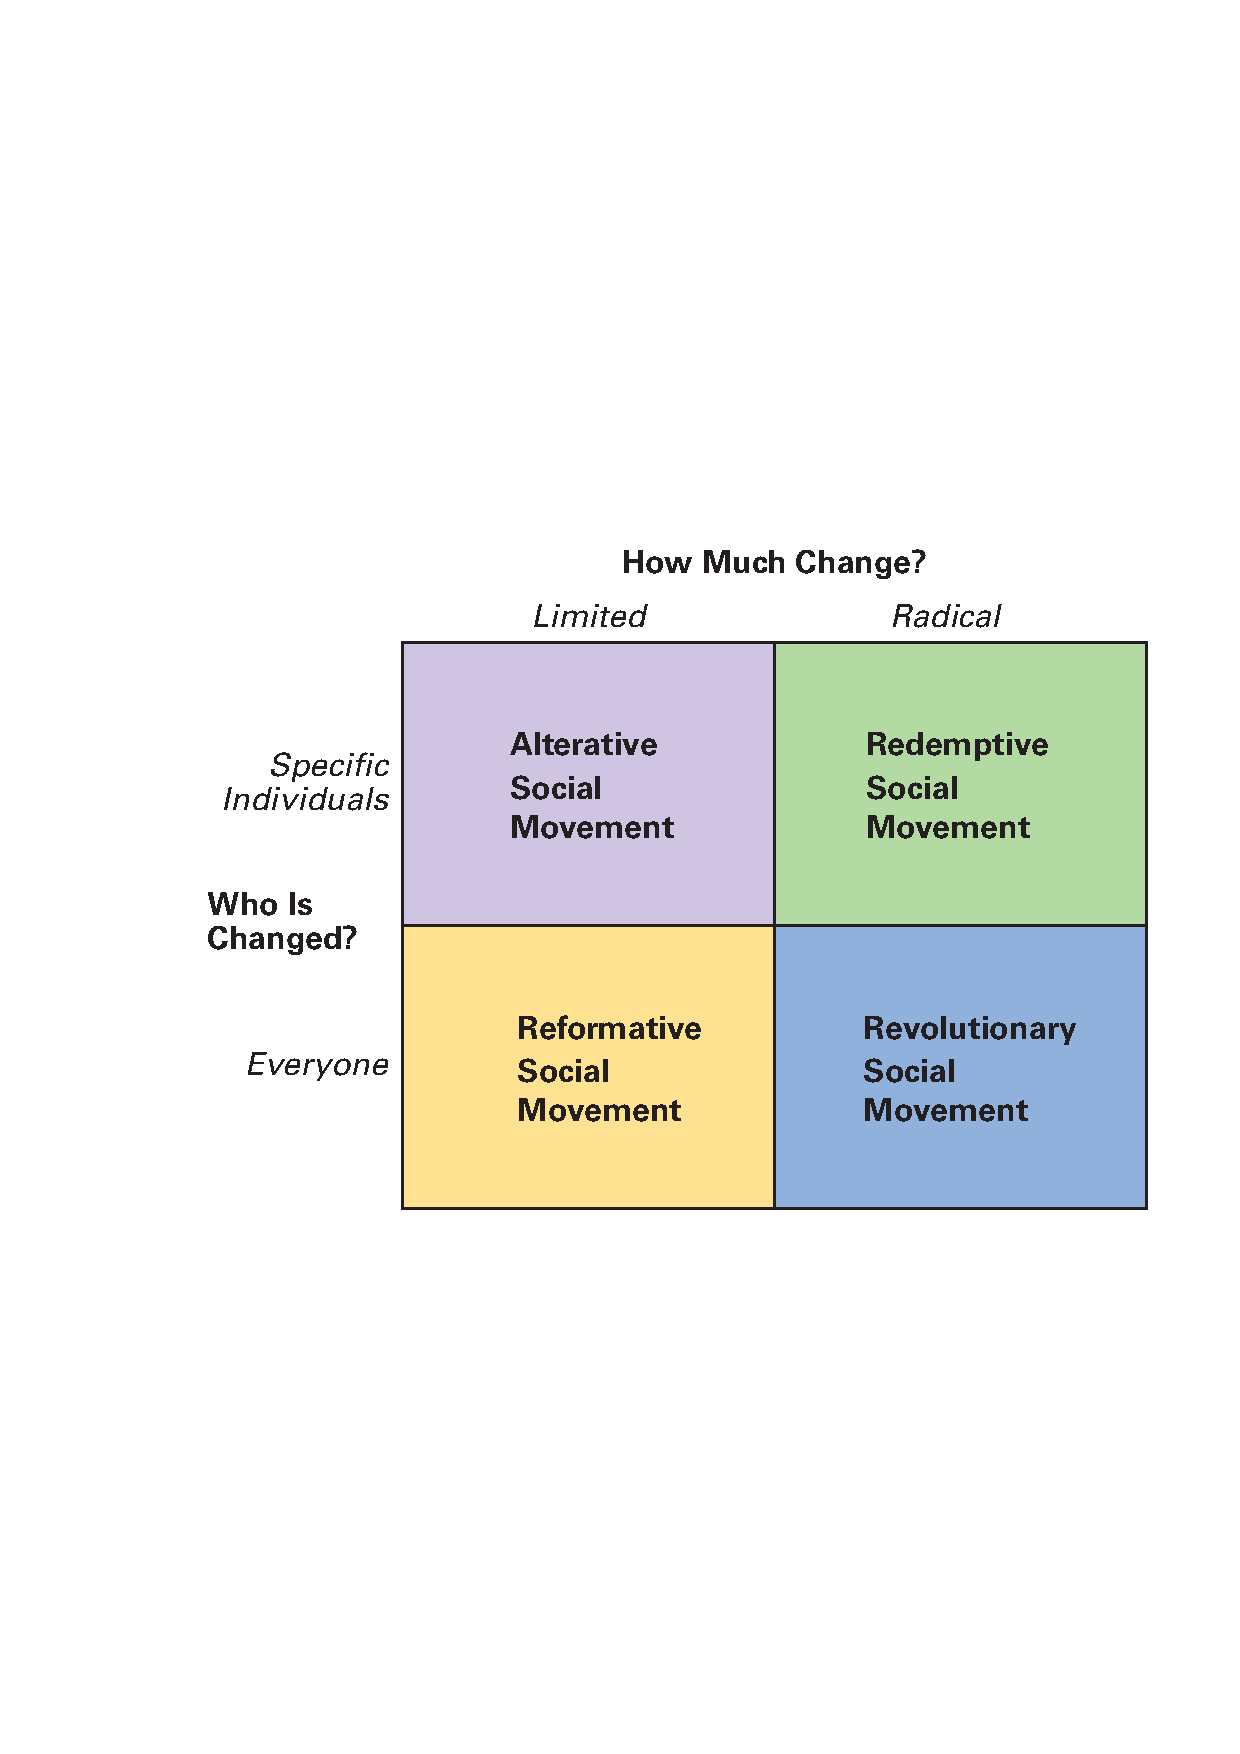
\includegraphics[width=0.9\textwidth]{assets/4_Types_of_SocMovements.pdf}
    	\caption{Types of Social Movements \citep[pg. 549]{Macionis12}
    	\label{fig:socmovements}}
	\end{figure}

\begin{enumerate}
	\item \textbf{Alternative Social Movement}: only affects a small portion of the population and results in minor changes to their life, keeping most of the status quo intact \citep[pg. 549]{Macionis12}.
    \item \textbf{Reformative Social Movement}: targets at a minor social change that influences the life of everyone. It usually works with the given political structure and can be either \textbf{progressive} (by actively promoting new social patterns) or \textbf{reactionary} (by opposing a specific movement for social change and trying to keep the status quo) \citep[pg. 549]{Macionis12}.
    \item \textbf{Redemptive Social Movement}: seek to help a specific group of people to change their life profoundly \citep[pg. 549]{Macionis12}.
    \item \textbf{Revolutionary Social Movement}: transformation of an entire society by rejecting current social institutions and proposes a new system \citep[pg. 549]{Macionis12}.
\end{enumerate}

Targeting only a subset of society or a specific individual usually occurs without the general public even noticing. To incite social change on a large scale requires making a specific claim. The process of \textbf{making a claim} is ``the process of trying to convince the public and public officials of the importance of joining a social movement to address a particular issue'' \citep[pg. 549]{Macionis12}. It typically starts with a small number of people supporting the claim, who tries to convince other members of the society to assist the case. If they can \textbf{gain mass media attention} they will likely get \textbf{recognized by public officials}, who may also speak out for the issue. In those situations the social movement will get stronger and stronger \citep[pg. 549]{Macionis12}. For our project, this is the stage of the social movements that online petitions appear to fit in -- they assist social movement organisers garner public attention.\par\vspace{0.2cm}

Sociologists have examined the motivations people have to join a social movement and came up with the following theories:
\begin{itemize}
	\item\textbf{Deprivation Theory}: members of the society that experience either absolute or relative deprivation -- relative means ``a perceived disadvantage arising from some specific comparison'' \citep[pg. 550]{Macionis12}, will likely start a social movement to right what they feel is wrong.
    \item\textbf{Mass-Society Theory}: people who are socially isolated might start or join a social movement to get a sense of social participation and importance. This usually takes place in impersonal, mass societies where people are more enthusiastic to form a common sense of community \citep[pg. 550f]{Macionis12}.
    \item\textbf{Culture Theory}: social movements are based on cultural beliefs and symbols that can be utilized to form a ``shared understanding of the world that legitimate and motivate collective action'' \citep[pg. 551]{Macionis12}. In addition to ``a sense of injustice ... people must come to believe that they are not able to respond to their situation effectively by acting alone'' \citep[pg. 551]{Macionis12}. Establishing symbols helps generate a common sense and form a community with strong beliefs and motivation to act. 
    \item\textbf{Resource-Mobilisation Theory}: states that the main success factors of a social movement are access to substantial resources like money, people, communication technologies, mass media and a positive public image. ``In short, any social movement rises or falls on how well it attracts resources, mobilizes people, and forges alliances'' \citep[pg. 552]{Macionis12}. To support this, the Internet can play an important role to help organize and mobilize many thousands of people through digital democracy, e.g. online petitions.
    \item\textbf{Structural-Strain Theory}: social movements start when people think their society has serious problems or does not meet their expectations. The social movement must have a clear message including a description of the problem, its causes and possible solutions to attract and maintain supporters in an organized way. Activities have to be coordinated and the success also depends on how political officials, the police and the military are reacting. \citep[pg. 553]{Macionis12}   
    \item\textbf{Political-Economy Theory}: social movements occur as a result of the current status quo that is failing political or economical needs for a group of the society  \citep[pg. 554]{Macionis12}.
    \item\textbf{New Social Movements Theory}: is a recent theory that shows that the focus of social movements is shifting away from the economical aspect to issues dealing with our social and physical environment -- including the environmental protection case. Unlike earlier theories, new social movements are handled on a global scope and deal with international affairs, e.g. global ecology, social standing of women and animal rights. Those movements are generally supported by people from the middle and upper-middle class due to their higher education level whereas economically driven movements are usually backed by people from the working class \citep[pg. 554f]{Macionis12}.
\end{itemize}
% subsection social change (end)
% End section: the big idea

\section{Methods}
\label{sec:methods}
To support the hypothesis that online petitions drive social change for environmental protection, we adopted a multimethod approach. The multimethod approach allows qualitative results (such as how people subjectively observed the impacts of online petitions) with quantitative data (such as how many supporters an online petition had, and how many countries were represented). The methods used include:
\begin{itemize}
 \item A \textbf{literature review} to first establish current theories regarding the online petitions phenomenon
 \item\textbf {Descriptive case studies} to observe online petitions and how they display characteristics found during the literature review.
 \item \textbf{Interviews} for qualitative analysis of possible reasons to make positive decisions in environmental petitions
 \item \textbf{Surveys} to determine the influence of online petitions on solving environmental issues
 \item \textbf{Web Site analysis} for quantitative analysis of typical users of online petition platforms like Change.org, detailed analysis of petitions related to environmental protection 
\end{itemize}
This section identifies first how the hypotheses were arrived upon and why these particular methods have been chosen to test them, then outlines the methods used to test them.

\subsection{From Testable Hypotheses to Methods}
\label{subsec:socialmethods}
In order to choose appropriate methods, inductive and deductive schools of thought were used to arrive upon testable hypotheses.
Inductive logical thought is the ``reasoning that transforms specific observations into general theory'' \citep[pg. 72]{Plummer11}. It is a bottom up approach that tries to understand facts at hand and come up with general theories to explain them. Inductive logical thought turned observations of successful online petitions on Change.org into the general theory that online petitions could represent an effective tool for digital democratisation.\par\vspace{0.2cm}
Following inductive logical thought is deductive logical thought, which involves ``reasoning that transforms general theory into specific hypotheses suitable for scientific testing'' \citep[pg. 72f]{Plummer11}. It is more of a top down approach, and sets the stage for scientific evaluation. It was deductive logical thought which lead to both the narrowing of ``online petitions are an effective tool for digital democracy'' to limit it to areas of environmental protection to improve testability, as well as to identify particular characteristics of online petitions which may explain why they appear to be effective: shareability, global reach, offering a premise for further media coverage, ease to hide failed petitions and so on. It also highlighted that it may indeed be correlation rather than causation, a critical hypothesis to examine.\par\vspace{0.2cm}

The methods must be appropriate to test the primary hypothesis of the paper:
\begin{itemize}
\item Online petitions drive social change in favour of protecting the environment.
\end{itemize}

\subsection{Measuring the connection between environmental problem petition victory and real decision}

Our goal for the inductive analysis is to measure the connection between environmental problem petition and victory on this problem. To achieve this goal we raise following research questions:
\begin{itemize}
	\item[\textbf{RQ1:}] What level of influence did the online petition have on the decision?
	\item[\textbf{RQ2:}] What are the main reasons decision-makers accept the petition?
	\item[\textbf{RQ3:}] What is the difference between expectations and results for petition starters?
%	\item[\textbf{RQ4:}] What are the motives of signers?  
\end{itemize}
\subsubsection{General description of surveys}
We will pick petitions for research using the following criteria:
\begin{itemize}
\item The petition must be reported as successful.
\item The online petition must involve an aspect of environmental protection.
\end{itemize}
An online petition marked as successful indicates it accomplished the goals of the petition starter, however whether the online petition itself caused the goals to be reached or some external factor caused the goals to be reached must be tested. The project goal is to test if an online petition is a plausible, effective tool of digital democracy which results in environmental protection, therefore the petition must be related to that purpose.\par\vspace{0.2cm}

To answer the RQ1 and RQ2 we must understand some other aspects of the online petition and those involved in the decisions which satisfied the online petition's demands. Those that deserve attention are:

\begin{itemize}
\item Were there any other supporting actions?
\item If they were, which role did they play in overall success of the online petition?
\item At what stage, if any, did mass media join the process?
\end{itemize}

We must consider this factors in evaluating the influence on the decision process. Hence, we will build a model to evaluate the significance of different aspects in decisions related to the online petitions. Our initial list of factors for the decision-maker to satisfy the requests of the online petition consist of:

\begin{itemize}
\item The petition was signed by many supporters.
\item The petition was featured in the media.
\item A higher authority demanded the issue be resolved.
\item A person in authority supported the case made by the online petition.
\item Actions of protest were held.
\item It was internal motivation without external influence.
\end{itemize}

We will use a 6-point Likert scale with answers:
\begin{enumerate}[start=0]
\item Disagree Strongly
\item Disagree
\item Tend to Disagree
\item Tend to Agree
\item Agree
\item Agree Strongly
\end{enumerate}

The Likert scale will capture the significance of the aforementioned factors. A Regression Analysis will be used to summarise the results. Also, after the exploratory phase (will be discussed later) we will decide if any Multivariate or Factor analysis will be needed.\par \vspace{0.2cm}

If the decision was made by a group we will aggregate the values for the group. In that case, we will get no more then 5 people from the group who made the decision to satisfy the request made by the online petition. If too few decision-makers agree to participate in our survey, it may be an indicator that petitions do not have influence on decision making processes. In that case, we will rely on the results of the survey for petition starters.\par\vspace{0.2cm}

To answer the RQ3 question we will perform a survey among online petition starters. We will ask petition starters two different points of the petition process: immediately after the petition starts, and within twelve months of their petition being granted 'successful' status. There is a risk that too few petitions will succeed from those that participated. In this case we will broaden the participant list for the second stage of survey by all successful petitions, not only those who attended on the first stage.\par\vspace{0.2cm}

Our initial list of the expectations to include in the survey for online petition starters are:

\begin{itemize}
\item The petition will be successful and will directly drive the decision.
\item The petition will support another activity online.
\item The petition will support another activity offline.
\item The petition will be noticed and supported by the media.
\item The petition will be noticed and supported by authorities.
\item The petition will be noticed and supported by environmental organisations.
\end{itemize}

Again, we will use a 6-point Likert scale for answers:

\begin{enumerate}[start=0]
\item Disagree Strongly
\item Disagree
\item Tend to Disagree
\item Tend to Agree
\item Agree
\item Agree Strongly
\end{enumerate}

The Likert scale will gauge the significance of the expectations of the petition starters. Similarly to the survey for decision makers, a regression analysis will be performed and the decision will be made if any Multivariate or Factor analysis will be needed.\par\vspace{0.2cm}

On the second stage of the survey we will paraphrase the states about expectations to the past tense, such that we have the following assessments regard the online petition:

\begin{itemize}
\item The petition has been successful and directly drove the decision.
\item The petition supported another activity online.
\item The petition supported another activity offline.
\item The petition was noticed and supported by the media.
\item The petition was noticed and supported by authorities.
\item The petition was noticed and supported by environmental organisations.
\end{itemize}

The list of results for the survey would be derived from the list of expectations. The same method for evaluation will be used to summarize the sample data, but additionally we will try to find the connection between expectations and results using ANOVA or MANOVA. We also intend to ask participants to answer the block of questions about the reason for the decision-maker to satisfy the petition requirement. We will use the form ``Do you agree that ... was the reason for the decision?''. If we will have enough answers from decision-makers we will perform a MANOVA to investigate whether the petition starters judgements about the reason their petitions were success may be a predictor of the reasons reported by the survey of decision-makers.

\subsubsection{Exploratory phase}
Qualitative research is exploratory and is useful when the researcher does not know the important variable to examine. This type of approach may be needed, because the topic is relatively new, the topic has never been addressed with a certain sample or group of people, or existing theories do not apply with the particular sample or group under study \citep{Morse1991}. To elaborate further on aspects of online petitions for consideration, an exploratory phase is required. This phase will also assist in ensuring the relevance of research questions.\par\vspace{0.2cm}

Firstly, we propose interviews with individuals who have started an online petition. We suppose that between three and five interviews with online petitions starters will be sufficient. For the type of interview, we have chosen semi-structured interview by phone or by teleconference (Skype, Google Hangouts etc.). This communication method is prefered to increase the response rate (due to the conveinence of using the phone versus organising face to face meeting). We suggest following questions to be answered as a basis, and deviations taken as necessary:

\begin{itemize}
    %\item Tell a brief story of 
    \item What is your background in environmental activism? Rationale: To start the interview with a topic easy for the interviewee to answer; to gauge the experience level of the campaigner.
    \item Why of creating the petition? Rationale: to capture motives for starting the petition.
    \item Was the publication of the online petition a primary action in your campaign? Rationale: to capture whether the online petition supplements a broader campaign.
    \item What were your expectations from the petition? Rationale: to capture whether the subject believed at the beginning that the online petition will result in action towards environmental protection.
    \item What other online promotional actions were done? Rationale: to capture other possible sources of influence on the final success of the online petition.
    \item What offline promotional actions were done? Rationale: to capture other possible sources of influence on the final success of the online petition.
    \item What sort of media coverage have you receieved for your campaign? Rationale: to capture the influence of the media on the campaign.
    \item What was, from your point of view, the main reason for the decision-maker to recognise your petition and respond to its requests? Rationale: determine if the subject believe the online petition caused the change, or some other factor.
    \item What can be other reasons for the decision-maker to accept a petition? Rationale: Cross-check the previous question.
\end{itemize}

A possible detailed plan of interview is written in \ref{subsec:interviewPlan} \par \vspace{0.2cm}
On the second stage of the exploratory phase we will perform from three to five interviews with decision-makers who responded positively to the requests of online petitions. The interview will similarly be semi-structured and conducted either over the phone or by teleconferencing. We suggest to begin with the following questions:
\begin{itemize}
\item How did you find out about the topic of petition? Rationale: determine the information sources that may have influenced the decision making process.
\item What other sources of getting know about environmental problem can be? Rationale: cross check the previous question.
\item How often do you judge the petitions (or how many times if it is not periodically)? Rationale: determine how receptive the subject is to petitions.
\item What were the main reasons why you fulfilled the request from the petition (from one to three)? Rationale: determine if the petition itself was a cause.
\item How did the number of signatures influence your decision? Rationale: determine if the number of supporters is a significant factor in online petition success.
\item What are some other sources of influence on decisions about environmental issues? Rationale: leading question to determine if pressure from online petitions is comparable to other sources of influence.
\end{itemize}

In the last stage of the exploratory phase we will form possible items for further research about expectations/results for the petition starters (taken from the surveys) and as well as reasons the decision-makers responded to the requests of online petitions (from the interviews).

\subsubsection{Statistical methods of the research}
In our research we are planning to use the following statistical methods:
\paragraph{Regression Analysis} In our Regression Analysis, sample data obtained as a result of the surveys is analysed by statistical methods to answer difference facets of the question -- do online petitions result in actions taken toward environmental protection? Regression analysis is commonly used in many research projects. An important instance of regression methodology called linear regression. These methods are the most frequently used in regression, and virtually all other regression methods build upon an understanding of how linear regression works. The goal of regression analysis is to summarise observed data \citep{Weisberg2005}. 

\paragraph{Multivariate analysis (MANOVA)} MANOVA is used in studies where research of more than one statistical variable is performed. In recent years, psychologists and other social scientists have devised models of behaviour on the basis of many different variables, all entered into the same equation. The goal of such analyses is to examine the extent to which variables predict one another, both individually and collectively \citep{GilesD2003}. A special case of MANOVA with only one dependent variable is called ANOVA.

\paragraph{Factor Analysis} Factor Anaylsis is a widely used statistical procedure in the social sciences. There is a general consensus that the technique is preferable to the Principal Components Analysis mainly because Factor Analysis seeks the least number of factors which can account for the common variance shared by a set of variables. Factors reflect the common variance of the variables, excluding unique (variable-specific) variance \citep{Krishnan2011}.

\subsubsection{Final notes}
In order to get more detailed results, the research can be extended in different ways. As well as environmental petitions other types of petitions can be examined, in which the connection between starting the petition and the decision can be found more easily or be more clear. Another way of extending the research is to analyse not only successful petitions, but also petitions which have failed or been closed. Such research can identify the reason of cancellation. For example, the starter may have found a more efficient way to solve the problem or the result of the petition did not met the expectations of the starter.\par\vspace{0.2cm}

Another option is to segment the results. One possibility is to segment by the number of signatures. The hypothesis as a result of the segmentation is that there can be different kinds of connection and influence depending on scale of petitions. Another option is to segment by scope of the petition. The possible values of the scope are: local, regional, national and global. The hypothesis of this segmentation is that for global issues significantly more effort and more complex promotional approaches are needed to achieve success.

\subsection{Deductive approach}
As we saw in The Big Idea section (chapter \ref{sec:bigIdea}) there are already various theories available of \textbf{digital democracies}, \textbf{environmental protection} and \textbf{social change and social movements}. Using the deductive approach we want to verify those of them that deal with \textit{using online petition tools to drive social movements for environmental protection}.\par\vspace{0.2cm}

There are two ways to verify those theories: we could use a classic approach by looking at each of the theories, searching for suitable parameters that we can use to validate the theory and then look for real-world data that might confirm the theory. On the other hand we can utilize a method that has been first introduced by Karl Popper named ``falsification''. This method does not try to prove a given theory by searching for facts that support it, but instead it tries to falsify the theory by looking for a negative case that will prove this theory wrong \citep[pg. 797]{Plummer11}.\par\vspace{0.2cm}
From chapter \ref{sec:bigIdea} we have the following theories that are of interest for our case study:
\begin{itemize}
    \item \textbf{Digital democracy}: Online petitions (and other tools of digital democracy) work effectively in a society that uses a pluralist model of political process.
    \item \textbf{Environmental protection}: Protecting the environment requires a global, combined effort and can not be solved on a local or national scope only. 
    \item \textbf{Social change and social movements}: Based on the new social movements theory, the online tools for creating global social change are mostly used and supported by people from middle (with a higher education level) and upper-middle class.
\end{itemize}

Based on those theories we formulate the following hypotheses to falsify them. Note, these are sub-hypotheses of the main hypothesis of this paper -- to test that: online petitions drive social change in favour of protecting the environment..

\begin{enumerate}
    \item Online petitions have an impact on the political decision making even if the society is not using a pluralist model. 
    \item Online petitions with either local or regional support have an impact on environmental protection.
    \item Online tools for digital democracy are used independently of class status, education level, nation, gender or age to drive environmental protection
\end{enumerate}

To validate those hypotheses we will have to capture and analyse data about usage statistics for Change.org as well as sample a set of successful petitions that deal with environmental protection to figure out about:

\begin{itemize}
    \item Demographics of users
    \item Origins of petition starters and supporters
    \item No. of supporters from same region
    \item No. of supporters from outside regions
    \item Scope of petition (local, regional, national or global)
    \item Social aspect of petition (economical, ecological, ethical or political)
    \item Social media coverage of petition (no. of supporters by channel)
    \item Offline support of petition (press or media coverage, protest, ...)
    \item Involved parties in offline support (NGOs, officials, lobbyists)
\end{itemize}

\subsubsection{Website usage statistics}
Online sites like Change.org can easily track and analyse their visitors by using tools that are available and known as ``Web Analytics''. They can use \textbf{Web logs} to access information that is related to the interactions between the web server and client, e.g. page name, IP address, browser, location of user and date time. Additionally, \textbf{cookies} can help to track returning visitors. More advanced tracking is possible with \textbf{JavaScript tags}, that the owner must include in his web sites. \par \vspace{0.2cm}
This information is usually only available to the owner of the web site and therefore it will not be available publicly and could not be used for our analysis. However, in addition to this private data of the web site there are also web usage metrics providers like Alexa.com \citep{Alexa14a} that make statistic data available to the public. Querying Alexa.com for Change.org \citep{Alexa14b} will give us information about the global or country-specific ranking of the site based on its traffic, demographics and geography information about its users, sites that users have visited just before and after they have looked at Change.org as well as the sites on the Internet that have links pointing to Change.org.  
\begin{figure}[H]
\centering
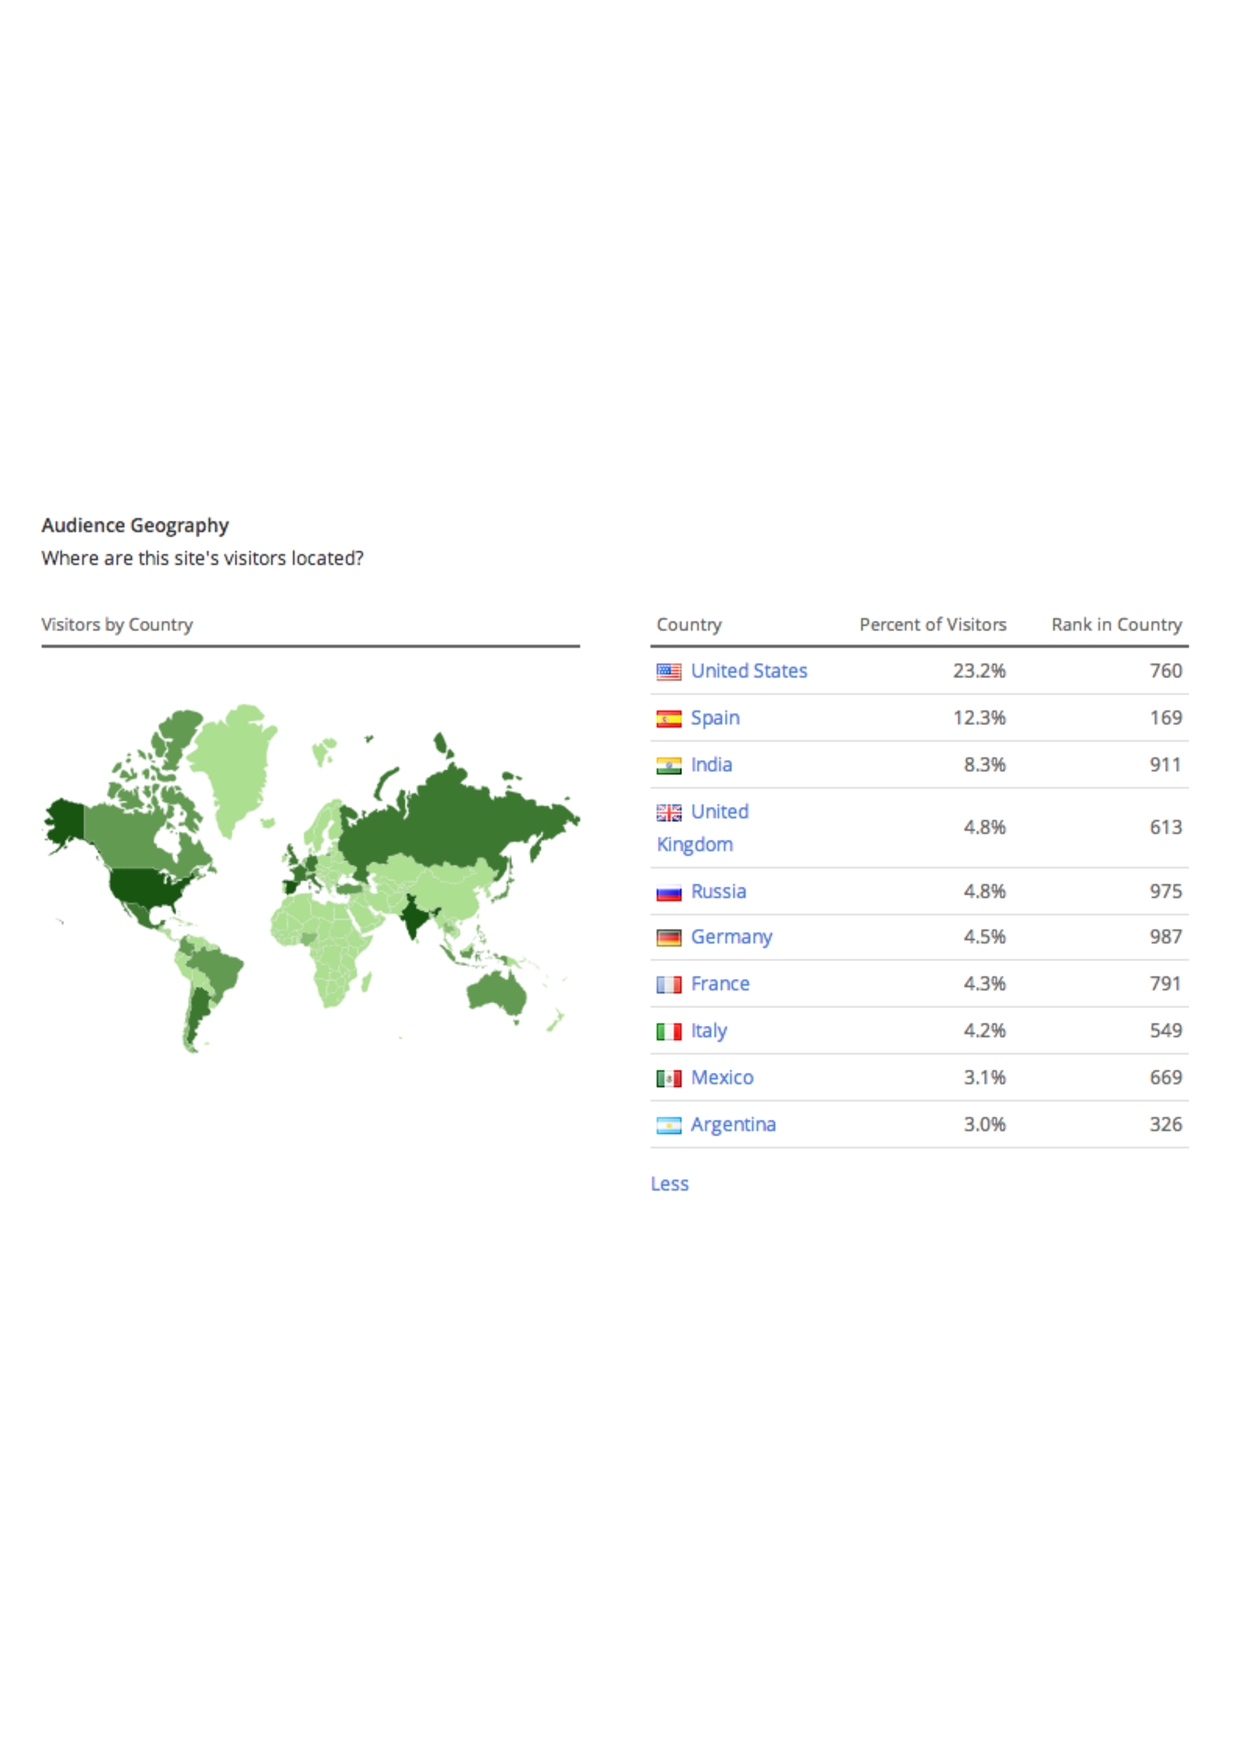
\includegraphics[width=0.9\textwidth]{assets/ChangeGeoStats.pdf}
\caption{Change.org Geography Statistics on Alexa.com}
\label{fig:change.org_GeoStats}
\end{figure}

We can see here that the Top 3 countries with active users on Change.org are:
\begin{enumerate}
\item United States
\item Spain
\item India
\end{enumerate}

Additionally, this statistic already shows that on a platform like Change.org not only developed Western countries are participating but also developing nations like India, Mexico or Argentina. This can be further related to hypothesis 1.

\begin{figure}[H]
\centering
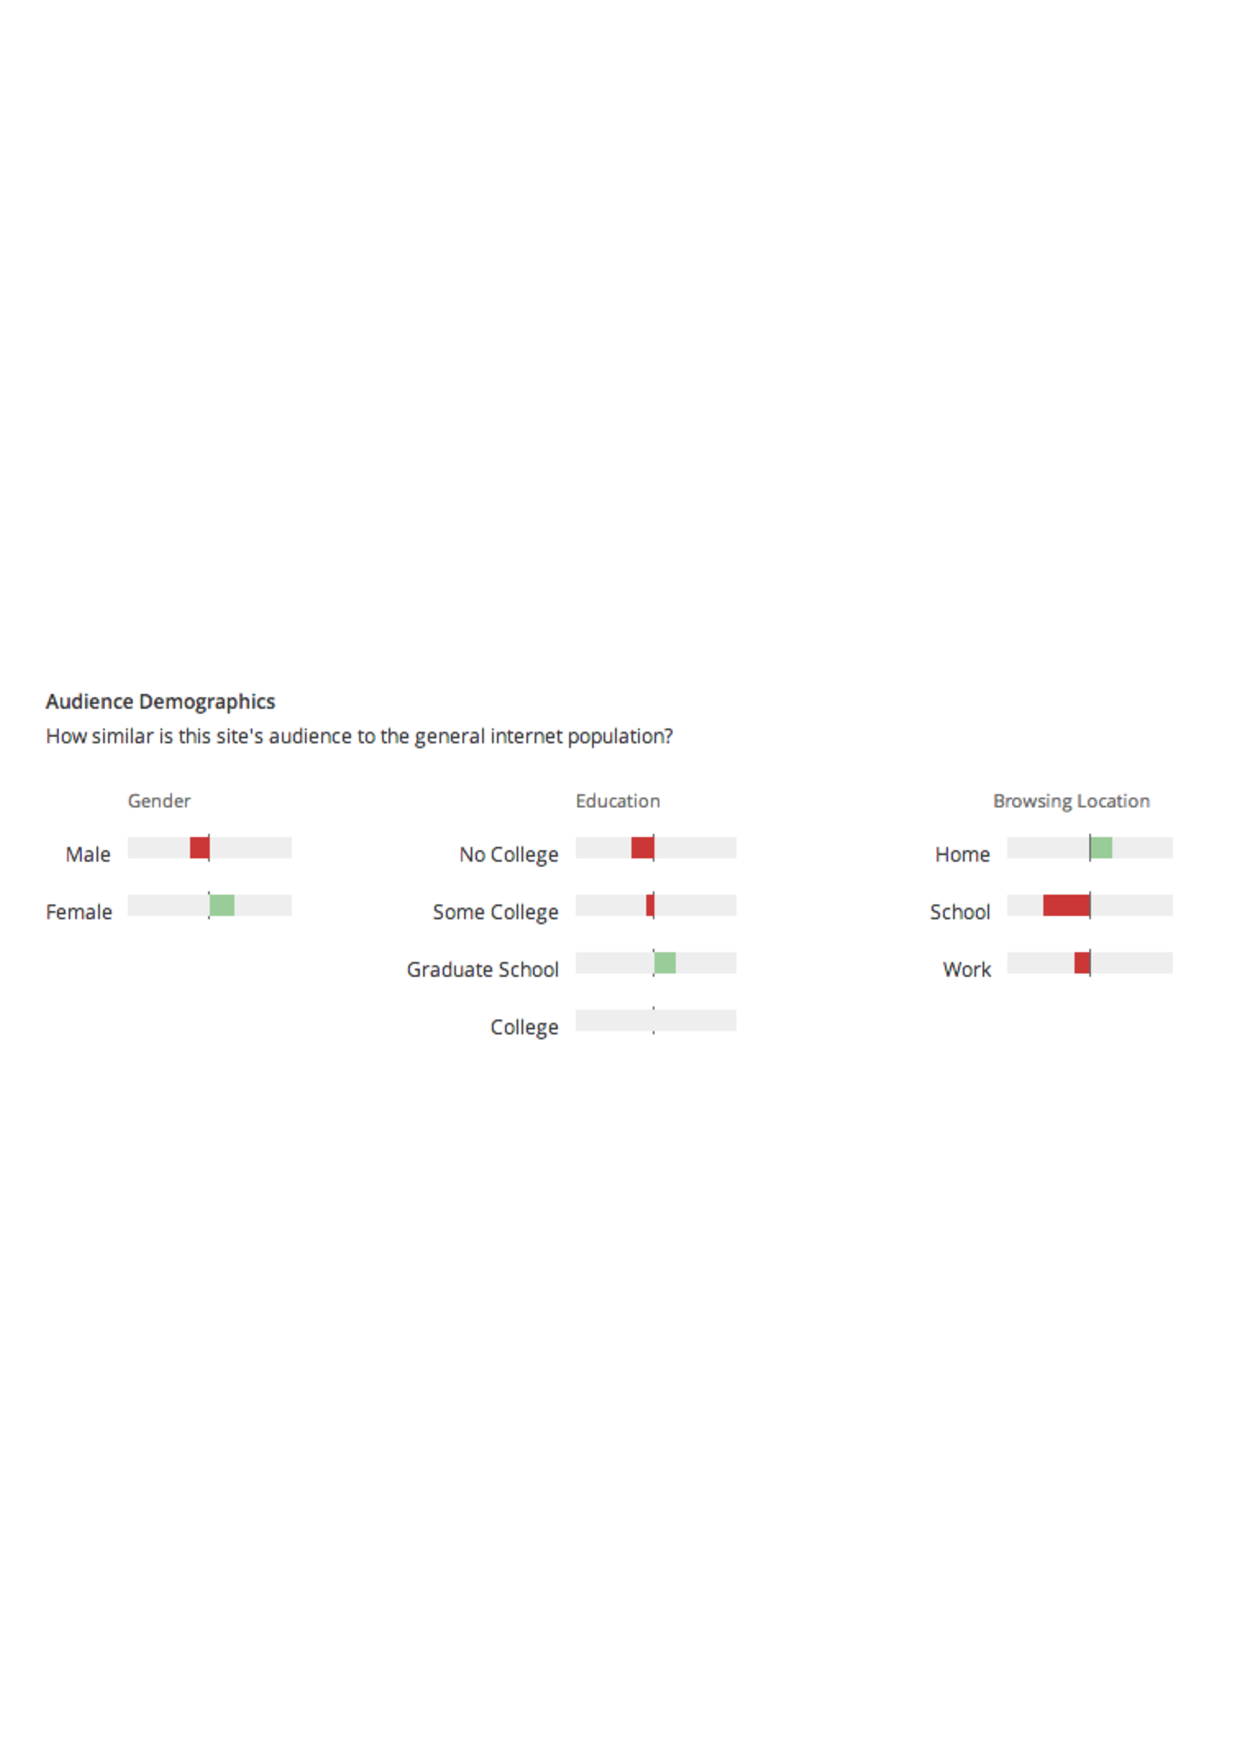
\includegraphics[width=0.9\textwidth]{assets/ChangeUserStats.pdf}
\caption{Change.org User Statistics on Alexa.com}
\label{fig:change.org_UserStats}
\end{figure}

Alexa.com offers additional statistics for the demographic information of the site's users when subscribed for a payed account. Without this account we can already make out some points. It appears like the third theory about the demographics of the people starting and joining new social movements holds. As the graphic shows there are more females than males and more people with higher education (college or graduate school) than undergraduate ones. This can be further related to our hypothesis 3.

\begin{figure}[H]
\centering
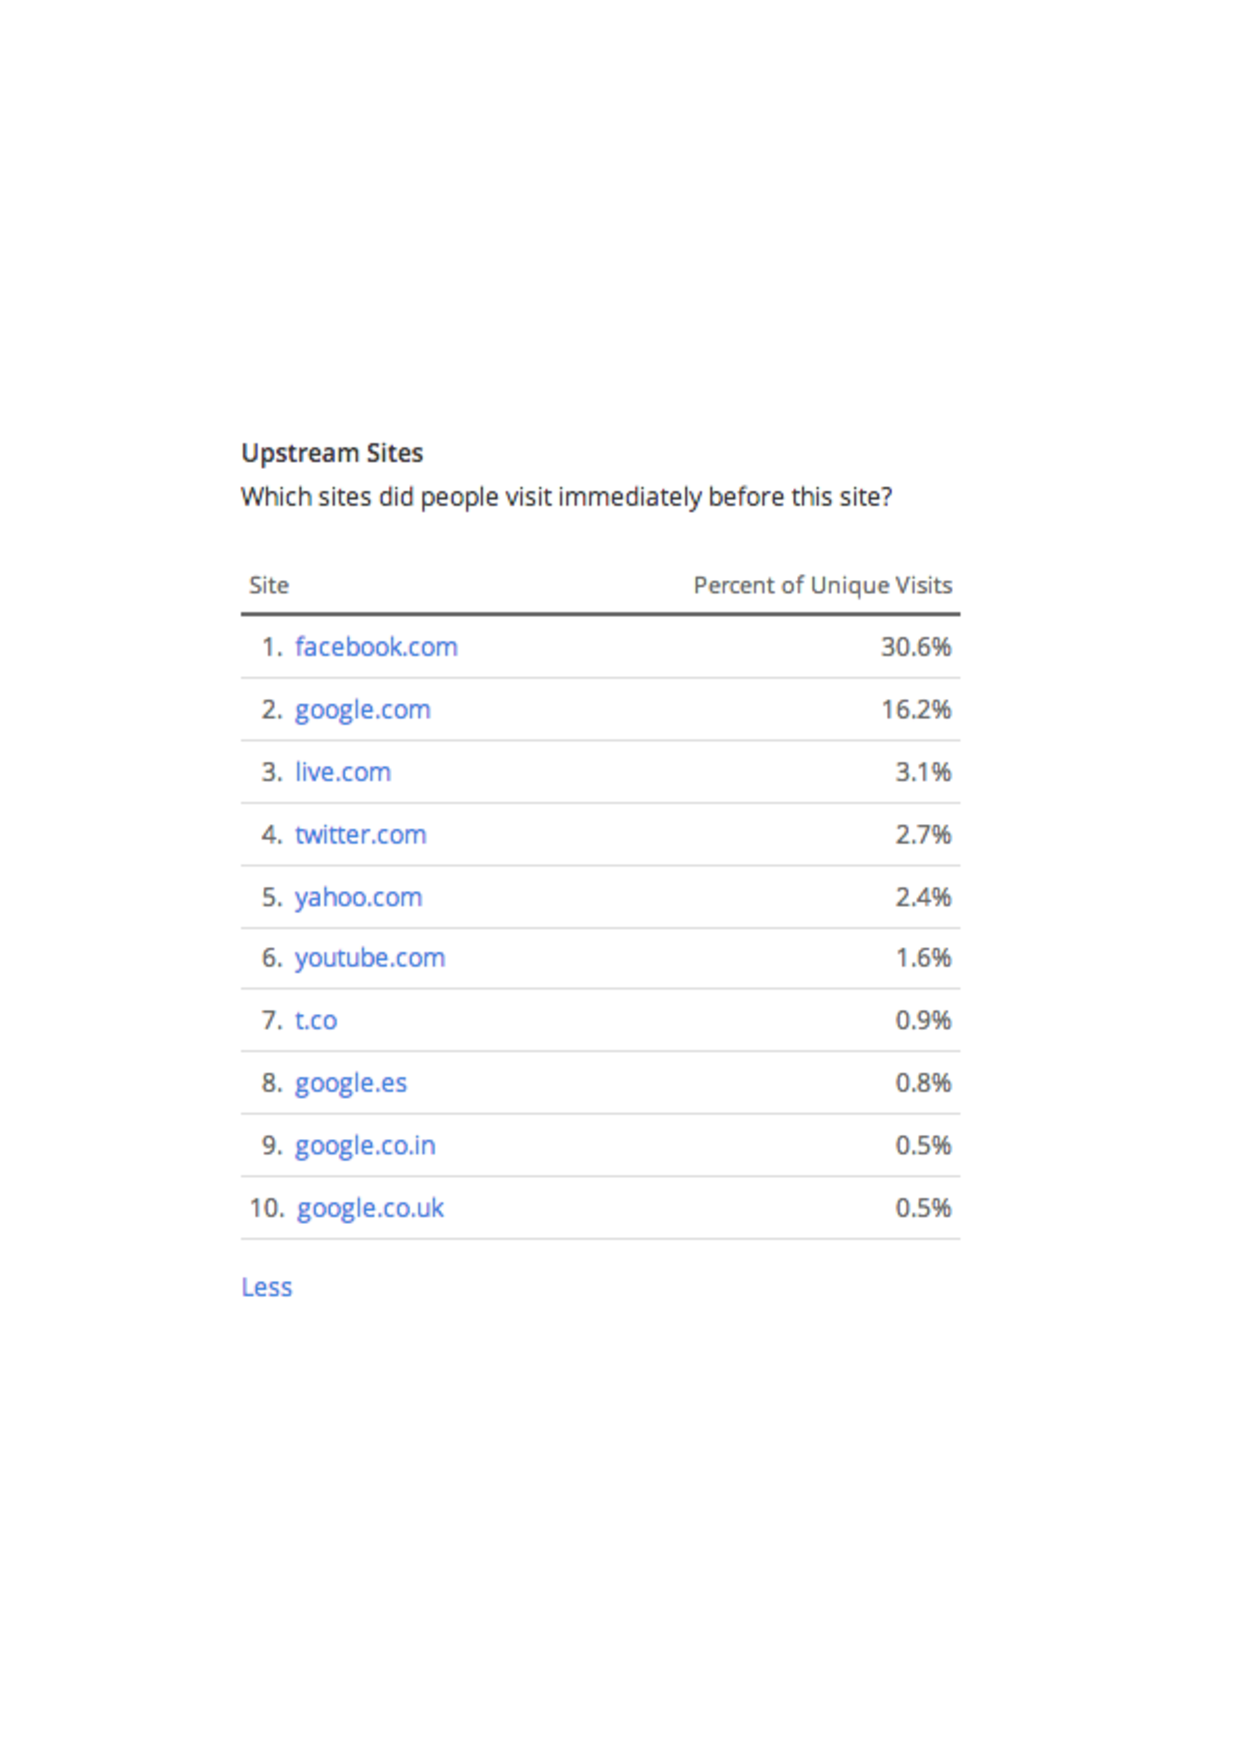
\includegraphics[width=0.6\textwidth]{assets/ChangeUpstreamSites.pdf}
\caption{Change.org Upstream Sites on Alexa.com}
\label{fig:change.org_upstreamSites}
\end{figure}

An important assumption we made for the success of an online petition is to reach a wider audience and connect the online actions with activities in the real-world. This statistic from Alexa.com gives us a list of sites that the users were on just before going to Change.org. We can conclude that these sites are mostly used to promote and refer to petitions from Change.org to a larger group of people to get their support and join it. As we see the Top 10 list is including Social Networks like Facebook, Twitter and YouTube as well as search engines like Google, Yahoo and Microsoft. This can be further related to our hypothesis 2.  

% subsection usage stats (end)

\subsubsection{Analyze petitions on Change.org}

More detailed information about the petitions and users on the platform Change.org is available via the Web API that the web site offers to developers \citep{Change14c}. So after registering and getting an access token you can easily query the Web API to get user and petition data via a REST-style interface. For users you can retrieve the following information: 
\begin{itemize}
\item \textbf{user\_id}: The ID of the user about which information was retrieved.
\item \textbf{name}: The full name of the user.
\item \textbf{location}: The full location of the user in English.
\item \textbf{city}: Residential city of the user.
\item \textbf{state\_province}: (If available) The standard abbreviation of the state or province of the user.
\item \textbf{country\_name}: Full English name of the country of the user.
\item \textbf{country\_code}: The two-letter code of the country of the user.
\end{itemize}

\citep{Github14a}.\par \vspace{0.2cm}

In addition to the user information the API also allows to query for petition records on the platform, petitions that has been started by a specific user as well as those that are supported by a specific user. A petition record will hold the following information:
\begin{itemize}
\item \textbf{title}: The human-readable title of the petition.
\item \textbf{status}: Possible values are open, closed, and victory.
\item \textbf{url}: The URL of the petition on Change.org.
\item \textbf{overview}: The overview text of the petition.
\item \textbf{targets}: The list of targets. (that is the list of addresses)
\item \textbf{letter\_body}: The body content of the petition letter to the target(s).
\item \textbf{signature\_count}: The petition's total number of signatures.
\item \textbf{image\_url}: (If available) The URL to the petition's image on Change.org.
\item \textbf{category}: (If available) The category that the petition is in on Change.org.
\item \textbf{goal}: (If available) The signature goal for a petition.
\item \textbf{created\_at}: The date and time the petition was created.
\item \textbf{end\_at}: (If available) The deadline for the petition.
\item \textbf{creator\_name}: (If applicable) The name of the petition creator.
\item \textbf{creator\_url}: (If applicable) The URL to the Change.org profile page of the petition creator.
\item \textbf{organization\_name}: (If applicable) The name of the organization that created the petition.
\item \textbf{organization\_url}: (If applicable) The URL to the Change.org profile page of the organization that created the petition.
\end{itemize}

\citep{Github14b}.\par\vspace{0.2cm}

Looking at this API description proves that we can query and access relevant user and petition information for our analysis. The absence of the \textit{age} attribute (though it is part of the profile on the Change.org website) prevents clustering the users based on their age and more in-depth analysis regarding the demographics of those creating online petitions. Based on the category information in the \textbf{petition} object we could find and filter those records that deal with environmental protection. Interestingly, it seems strange that the creator of the petition is optional at first, but this is more or less a technical trick as the creator of a petition could either be an individual or an organization.  

% subsection petitions on Change.org (end)

\subsection{Literature Review}
\label{subsec:literaturereview}
The literature review was conducted in order to create "a firm foundation for advancing knowledge" \citep[p. xiii]{webster2002analyzing}. This sections offers a brief overview of the current state.\par\vspace{0.2cm}

{Weblogs, traditional sources online and political participation: an assessment of how the internet is changing the political environment} by Zúñiga \textit{et al} looks at technologies to online petitions also having an effect on ``political discussion'' \citep{de2009weblogs}. While this paper covers a similar topic (although, not specific to environmental protection), it has focussed on a different technology: weblogs as opposed to online petitions. \textit{The Internet and Civic engagement} shows that, due to social media and blogs, politics is no longer limited to the ``well-off and well-educated'' \citep{smith2009internet}. Similarly to the \textit{Weblogs} article, we found that this article is highlighting that Internet technologies are indeed changing drivers of political action, however the importance of online petitions is not discussed.\par\vspace{0.2cm}

There were a few examples of literature that covers online petitions. The related work \textit{Digital Democracy through Electronic Petitioning} features a discussion of how online petitioning was used by the Scottish parliament to enhance public engagement \citep{macintosh2002digital}. Like the first two works, environmental protection was not a focus of this work. However, the tool discussed (the now off-line http://www.e-petitioner.org.uk/) seemed to serve a similar purpose as Change.org. Comparing and contrasting the effectiveness of Change.org to the Scottish Parliament's online petition could prove insightful as to how tools can be best applied to drive political action. Interestingly, it seems that the privately run Change.org has proven more popular than its government run counterparts. Lastly, \textit{Political Change in the Digital Age: The Fragility and Promise of Online Organizing} adopts a counter-position, that attention must be ``paid to the means of overcoming the difficulties of online organisation'' \citep{etling2010political}. Whereas, we have assumed, with tools such as online petitions, such difficulties have been mostly overcome.\par\vspace{0.2cm}

In summary, there are related works covering similar tools of digital democracy as well as online petitions. However, at least as far as we were able to determine, there is a space for an academic evaluation of Change.org and similar, `popular' online petition sites in relation to their effectiveness for environmental protection. Even more broadly, there also seems to be space for research investigating whether online petitions drive social changes in reality.

% subsection literature review (end)
\subsection{Primary case overview: Change.org}
\label{sec:PlatformsOverview}
% The following paragraph introduces our case study
We have chosen to do descriptive case studies. The Big Idea section articulates how digital democracies are driving social change for environmental protection in theory. Here we intend to mine real-world cases from Change.org and other on-line petition sites for 'abstract interpretations of data and theory development' \citep{casestudyResearch}.

\subsubsection{Brief history}
The site Change.org was launched on February 7, 2007. In 2008, Change.org cooperated with MySpace to ask the activists to submit policy ideas to the Obama administration \citep{Stirland2008}. During 2011, Change.org grew from 20 employees to 100 employees and offices on four continents\citep{Kristof2012}. Change.org has grown from six million users in the beginning of 2012 to more than 35 million users in May of 2013, and has become one of the largest and fastest growing petition platforms \citep{Empson2013}. In May 2013 the company has raised \$15 million investment from Omidyar Network \citep{Pozin2013}. In June 2014 the company announced a reach of more than 70 million users in 196 countries \citep{Change14a}. 
\subsubsection{Business model}
Change.org's business model is based on sponsored petitions. It is possible for the petition starter to pay for promotion of the petition among registered users. Most of the advertisers are non-profit organizations. Change.org claims that users will receive only those sponsored petitions the user interested in. Change.org pays close attention to the topics of petitions. They do not allow any hateful or discriminatory content. Another key point is that they never share private information without permission \citep{Change16}.\par\vspace{0.2cm}
One criticism of Change.org from users is that company is not clearly recognizable as for-profit organization.
\begin{quote}
The service is free, and with a name like Change.org the company even sounds like a not-for-profit. But it’s not. It was founded in 2007 and spent the better part of two years flailing around for a profitable business model until Rattray hit upon a clever approach. Change.org charges groups for the privilege of sponsoring petitions that are matched to users who have similar interests. For example, when a person signs a petition about education and clicks “submit,” a box pops up and shows five sponsored petitions on education to also sign. If a user leaves a box checked that says “Keep me updated on this campaign and others,” the sponsor can then send e-mails directly to that person. It’s not clear from the check box that your e-mail address is being sold to a not-for-profit. Rattray says an imminent site redesign will make the company’s business model more transparent. Change.org has 300 paying clients, including Sierra Club, Credo Wireless and Amnesty International, and its revenue so far this year is \$15 million.
\citep{Geron2012}
\end{quote}

\subsubsection{Victorious environmental cases}
Change.org claims over 6,000 victories and 50 million users. We investigated the site to find noteworthy cases of successful online petitions in support of the environment. The list of the cases can be found in \ref{subsec:VictoriousCases}. The minimum number of signers for considered cases is 259 and the maximum is 290,342. 

\subsection{Alternative platforms overview}
\subsubsection*{Avaaz.org}
Avaaz is an online campaigning organisation that is halfway between an NGO and a megaphone. Avaaz means "voice" or "song" in Persian \citep{Butler2013}.
Avaaz' mission is to close the gap between the world we have and the world most people everywhere want. Their community is unique in its ability to mobilize citizen pressure on governments everywhere to act on crises \citep{Avaaz2011}.\par\vspace{0.2cm}

The platform has 35 million members in 194 countries. Avaaz is \textbf{wholly member-funded}. They have no corporate sponsor or government backer, which may insist on an external agenda. They do not accept funds from governments or corporations.
\begin{quote}
Avaaz is both global and globalised and its approach is less bleeding-heart liberal than hard-headed pragmatist. It doesn't launch a campaign – to save fin whales from being butchered, or to free trapped migrant workers in Bahrain, or to bring peace to Palestine – because Patel, or the staff passionately believe in it (though they might). They launch a campaign that they think will fly. It's tried out on a sample of members and then they gauge the response. Patel says it's a way of ensuring that the members have the ultimate power, that they're the boss, not him.
\citep{Cadwalladr2013}
\end{quote}

\subsubsection*{Care2.com}
Care2 is a trusted social action network that empowers millions of people to lead a healthy, sustainable lifestyle and support socially responsible causes. Its content offering includes original stories, blogs and syndication partners covering a wide range of healthy lifestyle areas, and causes ranging from politics to human rights and animal welfare. By integrating relevant content with action opportunities such as petitions, pledges and daily actions \citep{Care22014}. Care2 owns and operates the site for petitions, \url{www.thepetitionsite.com}.\par\vspace{0.2cm}

Care2 is a profitable, privately funded company and a B-Corporation. The company's business model is focused on pay-per-action lead generation for non-profit organizations and CPM sponsorships for responsible consumer brands. As a B-Corporation or social enterprise, Care2 generates revenues by connecting individuals with nonprofits and businesses.\citep{Care22014} They anounced 25,9 Million members predominantly from US.

\subsubsection*{38degrees.org.uk}
38 Degrees is one of the UK's biggest campaigning communities, with over 2.5 million members. The organisation is "people-powered". They don't take money from political parties, government or big business, but \textbf{rely on donations from members}. 38 Degrees ask members to donate to support work or to fund a specific campaign or a specific action (e.g. to pay for the costs of organising a demonstration or putting up adverts). 38 Degrees has also received some money from charitable trusts and foundations. \citep{38degrees2014}
\par\vspace{0.2cm}
\begin{quote}
The campaigns that members are asked to support within 38 Degrees are simple one-step actions – signing a petition or sending a message to an MP – rather than more traditional, complex long-term campaigns.
This might mean that members take more than one discrete action towards achieving a positive outcome on the issue at hand, but the actions themselves are always meant to be simple, tangible steps toward that result. \citep{Puckett2011}
\end{quote}
As another example of activities, 38 Degrees organised debates with participation of UK parties to bring an in-depth look at the issues their members wanted to raise with the authors of each party's manifesto. \citep{Guardian2010}

\subsubsection*{Petitions.MoveOn.org}
In 2012, the liberal group MoveOn.org, one of the early successes of the digital political age, shifted to make member-driven petitions the center of its organizing efforts.\citep{Weiner2013}
\begin{quote}
Petitions can be started by any person or organization, not just MoveOn members. If a petition gets 20 signatures, MoveOn staff will send it to a small test group of members. If that group is enthusiastic, the petition will be sent to a larger group. If it continues to pick up steam, MoveOn staffers will work with the petitioners on running a campaign, including media training, phone calls, event organizing and fundraising help.
\citep{Weiner2013}
\end{quote}
MoveOn is entirely funded by small \textbf{donations from its members}. It consist of more than 8 million Americans.
\par\vspace{0.2cm}
Also, progressive state legislators and organizations such as Progress Now, Ultraviolet, Faithful America, the AFL-CIO, Free Speech for People, Social Security Works, Working Families Party, Color of Change, and the Organic Consumers Association have used MoveOn's petition website to give their campaigns a major boost.

\subsubsection*{Getup.org.au}
GetUp is an independent, grass-roots community advocacy organisation which aims to build a more progressive Australia by giving everyday Australians the opportunity to get involved and hold politicians accountable on important issues\citep{getup2014a}.
\par\vspace{0.2cm}
GetUp was founded in 2005 by a team of three Australians - Jeremy Heimans, David Madden and Amanda Tattersall. David and Jeremy are Australian graduates of Harvard University's Kennedy School of Government who have worked at the intersection of technology, new media and politics in the United States. David and Jeremy also co-founded Avaaz.org, a global online political community inspired by the success of GetUp and the US group MoveOn.org. Amanda Tattersall is a Sydney based community organiser who has founded a series of new social change organisations in Sydney and is known for her writing on civil society collaboration\citep{getup2014b}. 
\par\vspace{0.2cm}
GetUp is a \textbf{not-profit organisation} and relies on small donations to fund its work and in-kind donations from the Australian public. GetUp does not accept donations from political parties or the Government. It has over 630,000 members. In Anual report for 12/13 Financial Year the company reported \$ 4 061 664 donations \citep{getup2013}

\subsubsection*{Others}
Govermental organisations also have their own sites for petitions. The list of the most known is:
\begin{description}
\item[petitions.whitehouse.gov] "We the People". A section of the US White House website, launched in 2011.
\item[epetitionen.bundestag.de] A section of the Germany's Bundestag website, launched in 2005.
\item[epetitions.direct.gov.uk] A website for petitioning government and Parliament in the UK, launched in 2011.
\end{description}

\section{Conclusion}
\label{sec:conclusion}

In conclusion, it is still unclear whether online petitions definitely drive social change in favour of protecting the environment. There are some indirect evidences that this approach is effective, i.e. the fast growing of the popularity of this class of sites and the fact that such a authoritative movement like MoveOn.org decided to change its model to petition-driven. But for more evidence more research is needed.
\par\vspace{0.2cm}
This paper, thus far, has laid down the groundwork for further research into the issue of online petitions being used to drive social change in favour of environmental protection. As shown in the Big Idea section this is a complex issue that is surrounded by various factors that have to be taken into account. To deal with this complexity, we proposed a multimethod approach to produce more robust results. Research methods such as literature reviews, surveys interviews will assist in uncovering the motivations behind acts of environmental protection, especially whether or not they occurred as a direct result of online petitions. To support these findings, website statistics give us an opportunity to look at how online petition services are used today. Undoubtedly, as an increasing amount of activism is undertaken on the Web, determining which of the tools of digital democracy are the most effective will enable Web users around the world to best utilise the tools at their fingertips.









